\chapter{绪\hskip 0.4cm 论}
\label{chap1}

\section{研究背景}

随着移动定位技术、无线通信技术、普适计算技术的快速发展,以及智能手机的大量普及,人类进入了一个新的信息化时代——移动互联网时代。移动互联网已经融入到了交通、教育、娱乐、金融等人类生活的各个领域,对人类的发展有着极为深刻的意义。在早期的普通互联网时代,人们只能通过固定的PC终端连接到互联网,由于PC终端体积庞大,不具有便携性,极大的限制了互联网的发展。而在如今的移动互联网时代、智能手机的普及,使得人们可以不受时间和地点的限制,无论是在逛街还是旅途中都可以方便的连接到互联网。移动互联网的重要特性之一就是与地理位置的结合,这一特性使得移动互联网服务和应用更加丰富多彩,影响更加深远。

地理位置和移动互联网的结合促进了基于位置服务(Location-Based Service,LBS)相关应用的产生及快速发展,Foursquare、Loopt和新浪微博等在国内取得的成功足以彰显出这种新兴的LBS 隐藏着巨大的商业价值。在LBS应用中,用户通过定位设备(如GPS,传感器,RFID等)可以随时随地的获取到自身的当前位置。当用户需要LBS服务器(如大众点评)提供某种服务时,例如,娱乐信息服务(如查询距离我当前位置最近KTV、游戏厅或商店),导航服务(如查询当前位置到达华东师范大学的最短路径),交通服务(如查询“距离我最近的服务站”)。如图\ref{fig:communcationMode_pdf}所示:\ding{172}~移动用户首先通过定位设备(卫星)获取到自己当前的位置、\ding{173}~用户将自己的当前位置和查询需求(查找当前位置周围的KTV)发送给位置服务提供商、\ding{174}~位置服务提供商在收到用户的请求消息后,会根据相应的算法(如{$k$}邻近算法,KNN) 结合数据库选出和用户请求最为匹配的结果、\ding{175}~服务提供商将匹配结果返回给移动用户。简而言之,LBS 应用就是位置服务器根据用户提供的自身位置信息为用户提供的增值服务\cite{Mobile}。


\begin{figure}[H]
\centering
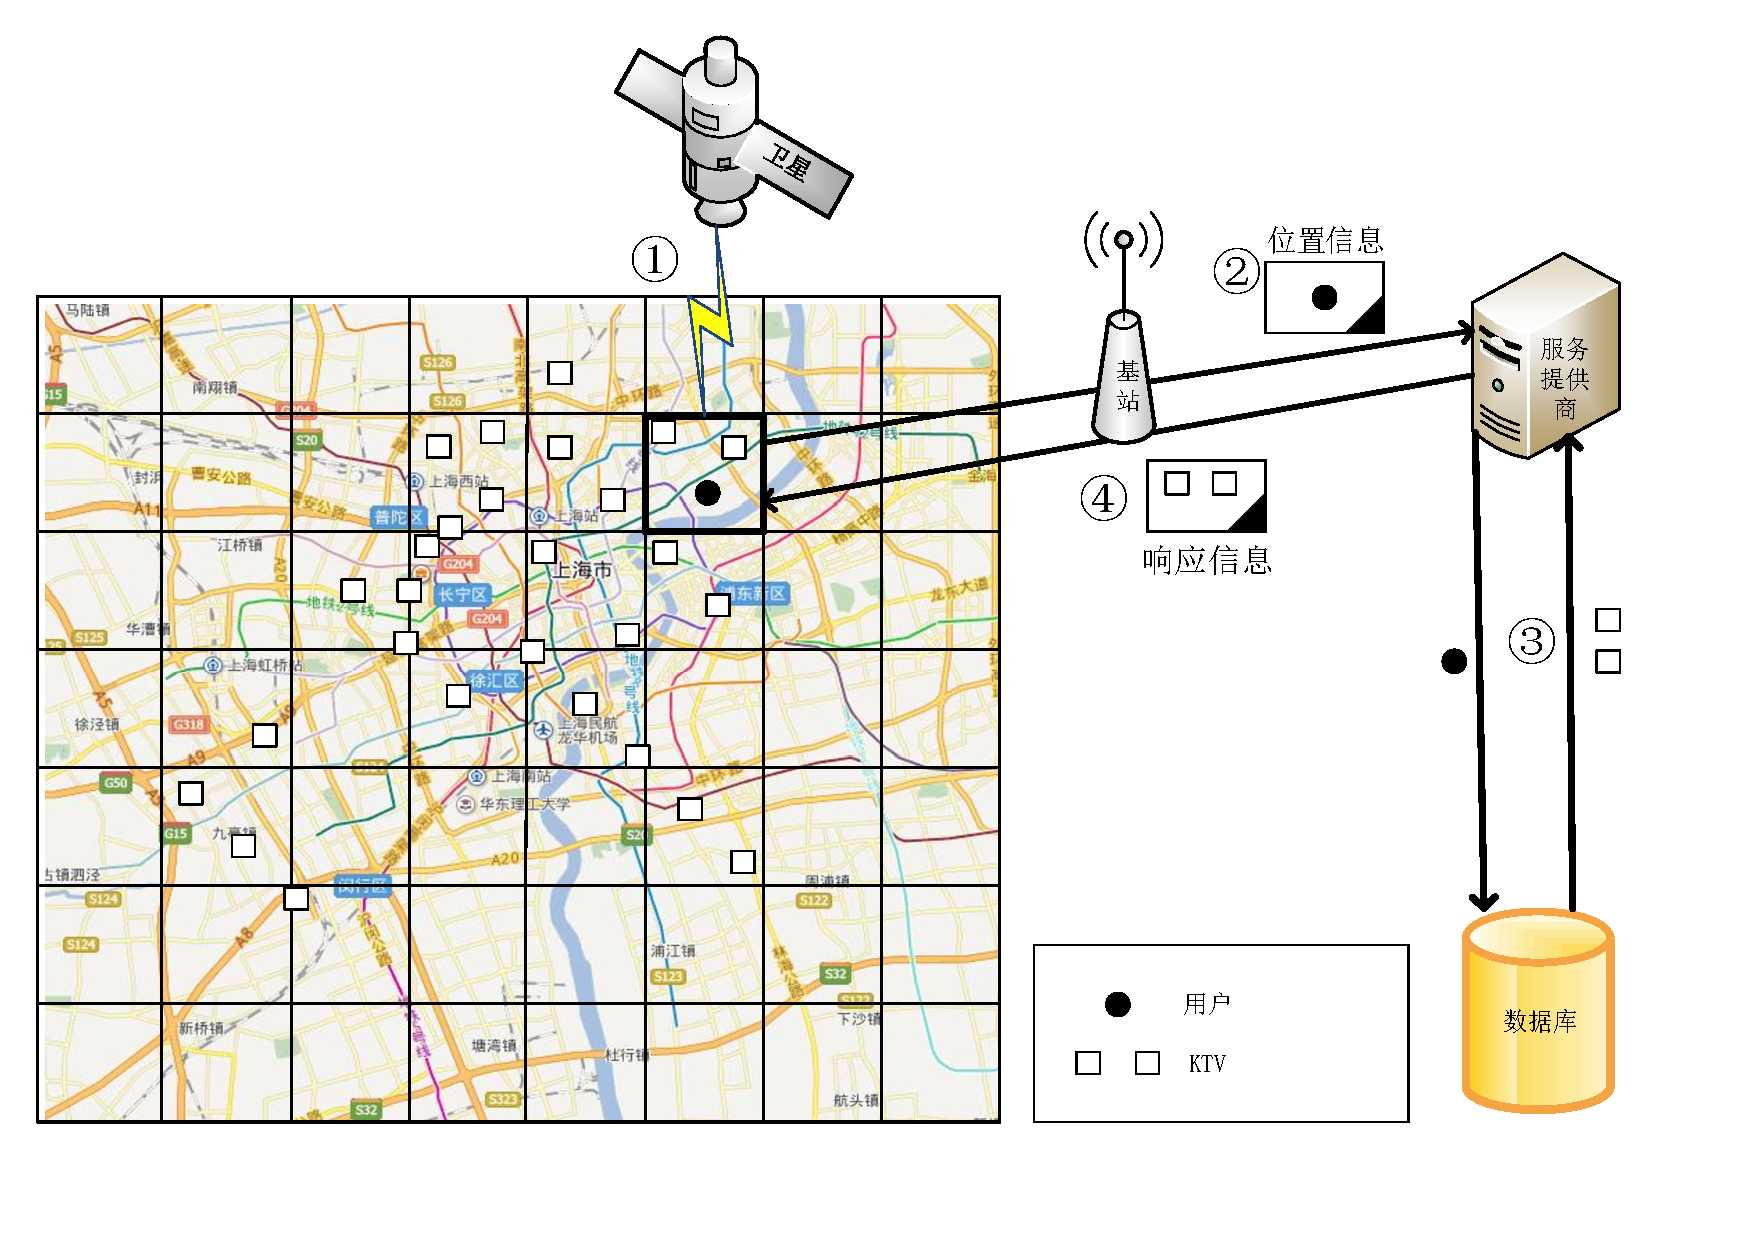
\includegraphics[width=15 cm]{fig/communcationMode.pdf}
\caption{基于位置服务通信模拟图} %\vspace*{-1.0cm}
\label{fig:communcationMode_pdf}
\end{figure}

在LBS应用中用户向LBS服务提供商提供自己的位置以及个人信息,服务器可以对这些数据进行统计归纳。这些统计信息无论是对个人还是对社会都有着极为重要的意义,个人可以通过这些信息挑选出最合适的餐馆就餐,到最合适的商场进行购物,利用位置的分布信息,可以避免上下班拥堵路段等。商户可以利用这些信息指定出更合适的销售计划,为不同的群体用户定制不同方案从而提供销量。政府可以利用这些信息进行道路交通的疏导,合理的部署公共基础设施等。可见,合法的利用位置信息对人们的生活,社会的发展有着重要的影响。


然而LBS应用的发展并非一帆风顺,LBS应用在给人们生活带来极大便利的同时,也对人们的隐私造成了一定的威胁。LBS服务提供商收集移动用户当前的位置信息,在此基础上执行空间查询,为用户提供位置服务。用户位置提供的越精确,LBS服务提供商返回的服务信息也越精确,但使得用户的位置暴露的越详细。这些位置信息也许揭露的不仅仅是用户的经度和维度,知道移动用户的位置信息也许可以知道用户在干嘛:正在参加会议还是听一场音乐会又或者是在哪里度假。当用户的位置信息被收集后,通过数据挖掘或分析,也许会得出用户的日常出行习惯以及出行路线等等。通常情况下,LBS服务提供商会将收集到的用户位置信息以一定的格式存放在数据库中,一旦存放这些数据的服务器被敌手攻破,那无疑是为攻击者窃取用户的隐私提供了极大的便利。

2010年微软在英国、德国、日本、美国以及加拿大进行了一份调查,调查结果显示94\%的消费者在使用LBS 应用时会考虑他们带来的价值,但在相同地调查中发现52\%人会关注他们的隐私是否存在泄露\cite{knn}。 位置信息的泄露对个人名誉以及人生安全都有严重的威胁。据国外媒体统计,78\%的小偷使用Facebook、Twitter对目标进行定位,从而确定主人是否在家中\cite{RSAInfo}。如何权衡服务质量和隐私保护之间的矛盾,已经成为LBS中位置隐私保护亟待解决的核心问题。
\section{隐私保护研究现状}
隐私保护一直是国内外学者研究的热点之一,研究内容主要有隐私保护数据的发布、用户空间位置的隐私保护。

数据发布是当前数据挖掘、数据分析到信息共享的一个重要环节。信息大爆炸以来,人们可以明显感受到大数据的来势凶猛。据相关调查显示,目前全球互联网每天的流量累计达1EB(即10亿GB 或1000PB),这意味着每天产生的信息量可刻满1.88 亿张DVD 光盘。海量数据如同一座未经开采的金矿,里面包含着无尽的信息与财富。但与此同时,也给数据的隐私带来了威胁。例如,通过对超市顾客的购买商品的记录进行分析,可以发现各种商品之间的关联(如啤酒与尿布),从而更好的进行货架的物品整理。然而在挖掘和分析的过程当中,不可避免的会使得顾客的信息暴露,从而可能造成顾客敏感信息的泄露。在文献\cite{sweeney}中,通过对性别、出生日期、住址等属性对选民登记表和隐藏了唯一标识符的医疗信息表进行连接操作,发现超过87\%的美国公民的身份可以被标识。因此,如何解决数据发布过程中存在的隐私泄露问题,已成为隐私保护研究的重点对象,也由此产生了一个新的研究领域——隐私保护数的发布。

数据发布的隐私保护技术主要有数据加密、数据匿名、数据扰乱等隐私保护技术。数据加密技术主要是基于密码学的隐私保护技术,文献\cite{group}利用群签名短发自主生成一系列伪签名证书来达到隐私保护效果,文献\cite{homomor}利用全同态加密方法使得服务器在不知道任何明文的内容的情况下可以在密文域上进行运算操作,得到的结果与在明文进行运算的结果相同。文献\cite{muticompute} 利用安全多方计算,可以保证在他人无法获得个人数据内同的情况下,计算出想要的结果。数据扰乱是一种数据失真的技术,Dwork等人提出了一种典型的数据扰乱的隐私保护模型—— 差分隐私模型\cite{differential},通过对发布的数据添加噪声进行随机扰动,使得在统计意义上攻击者无论具有何种背景知识,都不能判断一条记录是否存在原始数据表中。基于数据匿名的隐私保护技术主要是通过{$k$}-匿名技术\cite{kanonomy},在一个满足{$k$}- 匿名的数据库中,对于某一个准标识符({$QID$}, Quasi-Identifiers),值相同的记录至少有{$k$}条记录,因此通过{$QID$}去推断某一个目标记录的概率最多为{$1/k$}。

用户空间位置的隐私保护旨在保护用户当前的位置,近些年来,出现了很多位置隐私保护技术,在一定程度上保护了位置的隐私。这些技术主要包括:信息访问控制(Information access control)\cite{Myles}\cite{Youssef}、混合区域(Mix zone)\cite{Beresford}、 {$k$}- 匿名技术({$k$}-anonymity)\cite{Bamba}\cite{Chow}\cite{Mokbel}、假地址技术("Dummy locations")\cite{YiuML}\cite{Shankar}、 地理数据转(Geographic data transformation)\cite{HuH}\cite{Khoshgozaran}、 隐私消息恢复(Private Information Retrial,PIR)\cite{Ghinita}\cite{GhinitaPRIVE}。

基于访问控制,混合区域以及{$k$}-匿名LBS查询需要服务提供商或者中间件维护所有用户的位置。当服务器提供商/中间件由不可信方代理,受到的保护力度会相应的降低,因此容易受到第三方的攻击。在过去,私人数据无意间就暴露在互联网上。

{$k$}-匿名最初用在身份隐私保护。将{$k$}-匿名用在位置的隐私保护有点不适当,在位置的隐私保护概念中位置之间的距离是最重要的(身份隐私保护中身份之间的间隔是重要因素)。基于{$k$}-匿名的LBS查询精度很大程度上受到移动用户的密度和分布的影响,而这一影响因素已经超过了位置隐私保护技术所能控制的范围。

基于假地址的LBS查询需要移动用户随机选择一组虚假位置集合,通过移基站将虚假位置发送给LBS服务提供商并从服务商那里获得一份错误的报告。这将导致移动设备的通信和计算量过载。为了提高效率,移动用户也许减少集合中虚假位置的数量,但这将导致弱隐私性。

基于地理数据转换的LBS查询易受到访问模式攻击\cite{Williams},因为相同的查询总是返回相同的加密结果。例如,LBS服务提供商可以观察返回密文出现的频率,依靠数据库内容的相关背景知识,可以根据出现频率匹配出最有可能的明文结果,从而得到相关的查询信息。

基于PIR的LBS查询提供了很强的密码保障,通过数据加密使得服务器无法得到用户位置的信息,且能对用户的请求提供正常的服务。相比于之前的位置隐私保护技术,PIR技术对位置隐私保护的更加的安全,从理论上完全杜绝了敌手的攻击。


\section{本文工作与主要贡献}

本文以海量出租车轨迹数据为研究对象,基于已有研究成果,以智能打车推荐为应用目标,建立对轨迹数据的分布式处理框架和挖掘分析系统,并实现在线的查询与推荐服务。解决的问题包括:轨迹预处理、轨迹数据聚类、轨迹数据查询、预测和推荐模型建立等多个方面。
本文主要的研究工作内容如下:

\paragraph{对轨迹数据的分布式处理}

在对轨迹数据进行挖掘和分析的之前,数据的预处理工作能够提高模型准确度并辅助模型抽取出所需数据,通常包括对数据的降噪处理和过滤、轨迹数据到路网的映射等。鉴于轨迹数据的数据规模,并行的数据处理策略能够大大提高对批量历史数据处理的效率,本文工作中建立基于Map-Reduce的通用轨迹处理框架,实现在不同采样密度下优化的路网匹配算法,并将分布式处理框架应用于数据过滤、路网匹配、特征抽取等轨迹数据处理的多个关键阶段。

\paragraph{兴趣点和兴趣区域挖掘}

兴趣点和兴趣区域通常作为推荐元素向用户推荐,在不同的挖掘任务中,根据推荐的目标不同采用的方法也不同,聚类是发现轨迹数据特征的最常用方法之一,而对于时空特性明显的地理位置数据,聚类算法的设计、度量方法的选择、数据查询结构等均是该部分的主要研究内容。本文以打车推荐为目的,重点讨论采用基于密度的聚类方法对候选扬招点和热门目的地的挖掘方法。

\paragraph{出租车扬招推荐服务和候车时间预测}

基于位置的服务泛指一类利用定位技术获得当前位置信息,再通过无线网络得到某项服务的技术,能够为大量普通用户提供服务。利用历史出租车轨迹数据,我们可以为用户提供智能出行建议,减少用户行程中浪费不必要的时间。本文基于多种模型对不同路段出租车空车到达时间进行建模,利用兴趣点挖掘技术提供备选扬招点和目的地方案,建立预测准确、推荐合理的扬招点推荐系统,并提供查询应用服务。


\paragraph{本文主要贡献如下:}

\begin{itemize}
	\item 建立了基于Map-Reduce的分布式轨迹处理框架,并在此框架下实现了轨迹预处理和优化的路网匹配算法。
	\item 采用基于密度的聚类方法发现兴趣点和兴趣区域,从而找到备选扬招点和热门目的地。
	\item 实现了智能出租车出行推荐系统,该包含了数据预处理、路网匹配、特征抽取、路段聚类、在线预测、查询推荐等多个模块,完成了基于泊松过程、线性回归等的出租车等待时间预测算法。
	\item 提供在线扬招点查询和推荐应用,能够支持多种客户端实时的请求相应。
\end{itemize}

\section{组织结构}

第2章中回顾基于位置的服务的发展以及与本文工作相关的研究进展;第3章中介绍了本文实现的分布式轨迹数据处理框架,并具体阐述了本文采用的路网匹配方法和实验效果;为了实现后续的基于位置的打车推荐服务,第4章中介绍了利用轨迹点的聚类方法进行兴趣点和兴趣区域的挖掘,包括关键辅助索引结构和优化的基于密度的聚类算法;第5章基于前面的轨迹数据和聚类结果,实现了对扬招点和目的地的推荐应用,其中,重点介绍了对候选扬招点候车时间的预测模型,以及在线的查询和推荐算法。第6章总结全文,对后续的研究工作进行展望。

